\documentclass[10pt]{beamer}

\usetheme[progressbar=frametitle]{metropolis}

\usepackage{booktabs}
\usepackage[scale=2]{ccicons}
\usepackage{graphicx}

\usepackage{pgfplots}
\usepgfplotslibrary{dateplot}

\usepackage{xspace}
\newcommand{\themename}{\textbf{\textsc{metropolis}}\xspace}

\title{Artificial neural network-based photovoltaic
maximum power point tracking techniques}
\subtitle{A modern beamer theme}
\date{\today}
\author{Md. Samiul Haque Sunny}
\institute{Khulna University of Engineering \& Technology}
\titlegraphic{\hfill
\includegraphics[height=1.5cm]{logo}}

\begin{document}

\maketitle

\begin{frame}{Table of contents}
  \setbeamertemplate{section in toc}[sections numbered]
  \tableofcontents[hideallsubsections]
\end{frame}

\section{Renewable Energy \& PV Cell}
\begin{frame}{What is renewable energy?}
Renewable energy is generally defined as energy that is collected from resources which are naturally replenished on a human timescale, such as sunlight, wind, rain, tides, waves, and geothermal heat.
\end{frame}

\begin{frame}[allowframebreaks]{Solar Energy and PV Cell}

\begin{alertblock}{Solar Energy}
Solar energy is radiant light and heat from the Sun that is harnessed using a range of ever-evolving technologies such as solar heating, photovoltaics, solar thermal energy, solar architecture and artificial photosynthesis.
\end{alertblock}

\begin{exampleblock}{Photovolatic Cell}
A solar cell, or photovoltaic cell (in very early days also termed "solar battery" – a denotation which nowadays has a totally different meaning, see here), is an electrical device that converts the energy of light directly into electricity by the photovoltaic effect, which is a physical and chemical phenomenon.
\end{exampleblock}

\framebreak 

\begin{figure}
		\centering
		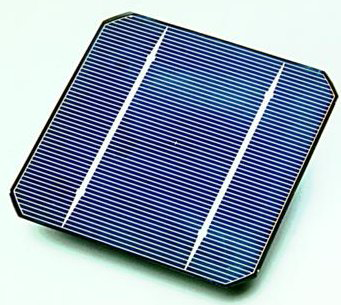
\includegraphics[width=0.6\linewidth]{pvcell.png}
        \caption{Figure of a PV Cell}
        \label{fig:pvcell}
\end{figure}
	
\end{frame}

\begin{frame}{Diode Model of PV Cell}
One basic equivalent circuit model in common use is the single diode model in following figure \ref{fig:diodemodel}

\begin{figure}
	\centering
    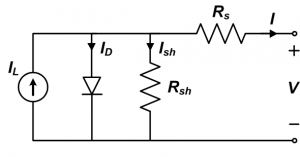
\includegraphics[width=0.6\linewidth,height=4cm]{diodemodel.png}
    \caption{Diode model of a PV cell}
    \label{fig:diodemodel}
\end{figure}

\end{frame}

\begin{frame}{Characteristics curve of Diode Model}
PV Cell I-V Characteristic Curve is shown below in figure \ref{fig:charCurve}
\begin{figure}
	\centering
    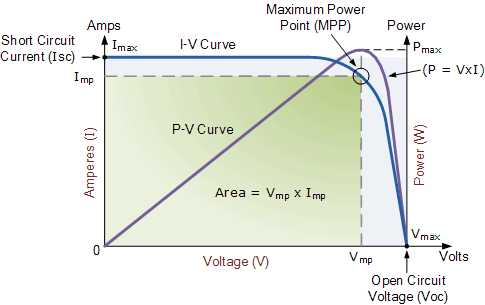
\includegraphics[width=0.6\linewidth]{alt120.png}
    \caption{I-V Characteristic curve of a PV Cell}
    \label{fig:charCurve}
\end{figure}
\end{frame}

\begin{frame}{Maximum power point tracking (MPPT) and PV Cell}
\begin{alertblock}{MPPT and PV Cell}
Maximum power point
tracking (MPPT) is a technique that charge controllers use for
PV solar systems to employ and maximize power output.
Maximum Power Point Tracking is a digital electronic
technique.
\end{alertblock}

\begin{exampleblock}{How MPPT Works}
After getting the output from the panel the charge
controller compares it to the battery voltage. From the
compared value it finds out what is the best power for which
panel can put out to the charge the battery. With this value and
converting it to the best voltage we get the maximum ampere
into the battery.
\end{exampleblock}

\end{frame}

%
% Boost converter
%
\begin{frame}[allowframebreaks]{Boost Converter}
\begin{alertblock}{What is a Boost Converter?}
A boost converter (step-up converter) is a DC-to-DC power converter steps up voltage (while stepping down current) from its input (supply) to its output (load).
\end{alertblock}

Figure \ref{fig:boostConvCkt} shows a typical circuit diagram of a boost converter.

\begin{figure}
	\centering
    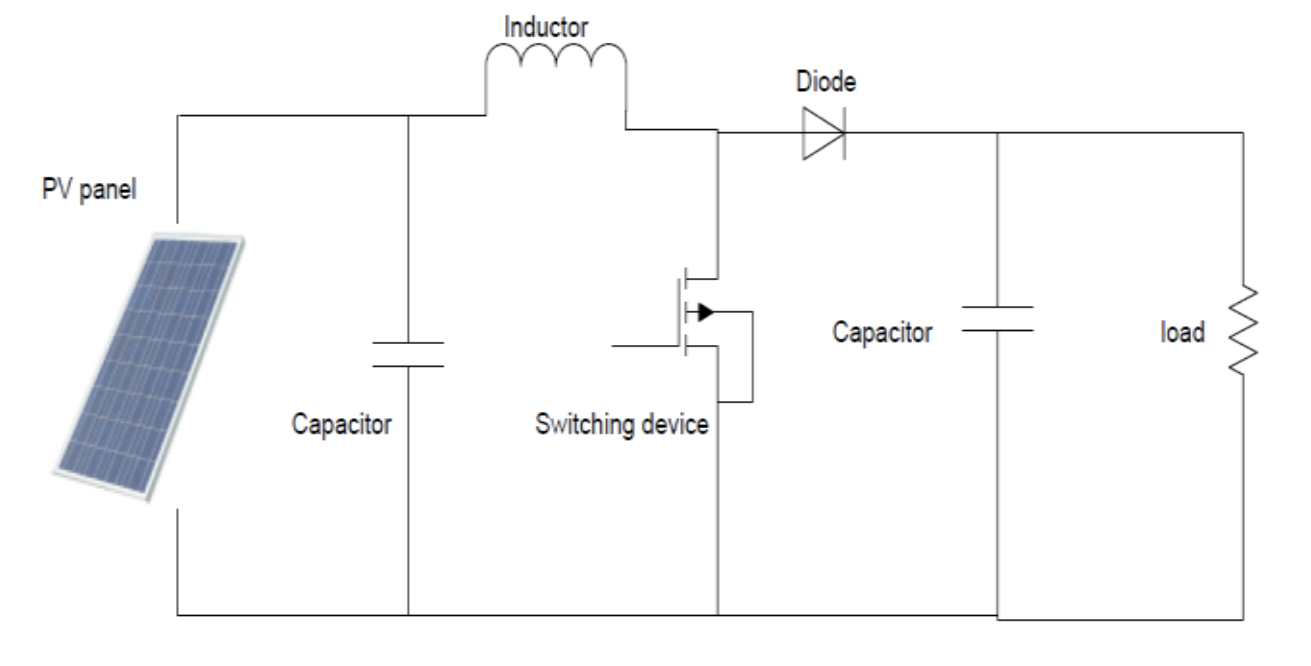
\includegraphics[width=.6\linewidth, height=4cm]{boostconverter.png}
    \caption{A typical circuit diagram of a boost converter.}
    \label{fig:boostConvCkt}
\end{figure}


\framebreak 

\vspace{1cm}
\begin{figure}
	\centering
    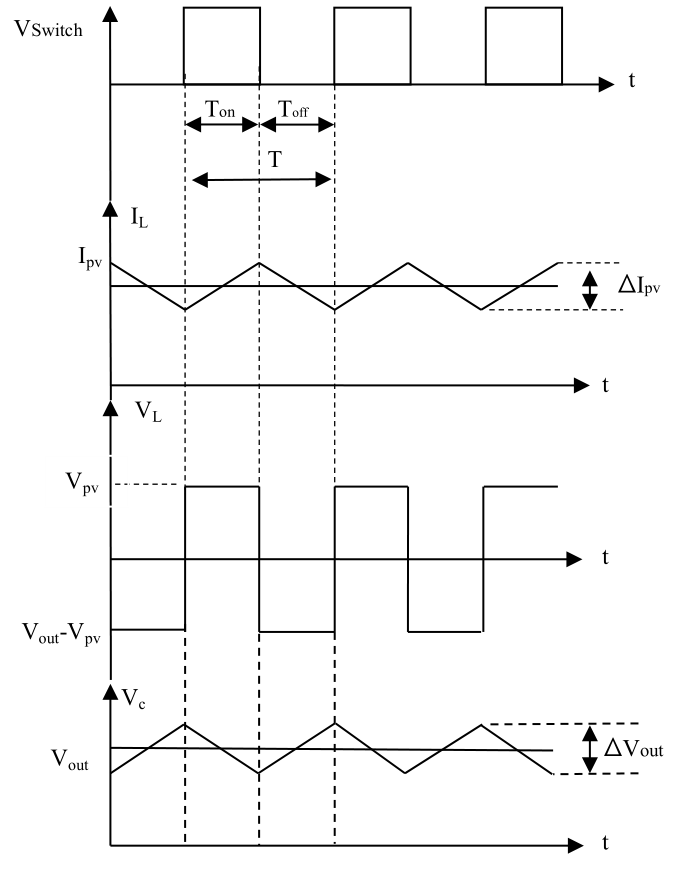
\includegraphics[width=.6\linewidth, height=6cm]{boostconvertergraph.png}
    \caption{Typical forms wave of boost converter.}
    \label{fig:boostConvWave}
\end{figure}

\end{frame}

\section{Artificial Neural Network}

\begin{frame}{An Artificial Neuron Model}
An artificial neuron is a mathematical function conceived as a model of biological neurons. Artificial neurons are the constitutive units in an artificial neural network. 

\begin{figure}
	\centering
    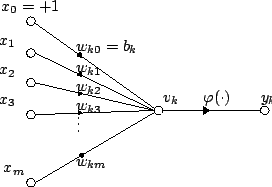
\includegraphics[width=2.5cm, height=2.5cm]{Artificial_neuron.png}
    \caption{Figure of an Artificial Neuron}
\end{figure}
\end{frame}

\begin{frame}{Feed forward Artificial Neural Network}

\begin{exampleblock}{What is an artificial neural network?}
An artificial neural network is an interconnected group of nodes, akin to the vast network of neurons in a brain. Here, each circular node represents an artificial neuron and an arrow represents a connection from the output of one neuron to the input of another.
\end{exampleblock}

\begin{figure}
	\centering
    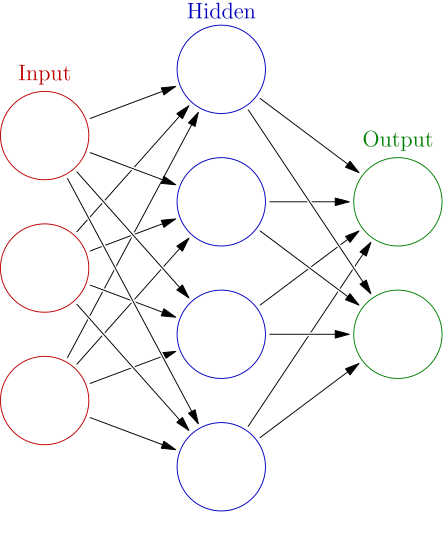
\includegraphics[height=4cm]{neuralnet.png}
    \caption{A Feed forward Artificial Neural Network.}
\end{figure}

\end{frame}

\subsection{Why ANN was chosen}

\begin{frame}{Why ANN was chosen for MPPT technique}

Artificial Neural Network (ANN) algorithms feature several capabilities such as 

\begin{enumerate}
	\item{Off-line training}
    \item{Nonlinear mapping}
    \item{High-speed response}
    \item{Robust operation}
    \item{Less computational effort}
    \item{Compact solution for multi-variable problem}
\end{enumerate}

\end{frame}

\section{Classification of ANN based MPPT Techniques}

\begin{frame}{ANN Input Nature}
	\begin{figure}
    	\centering
        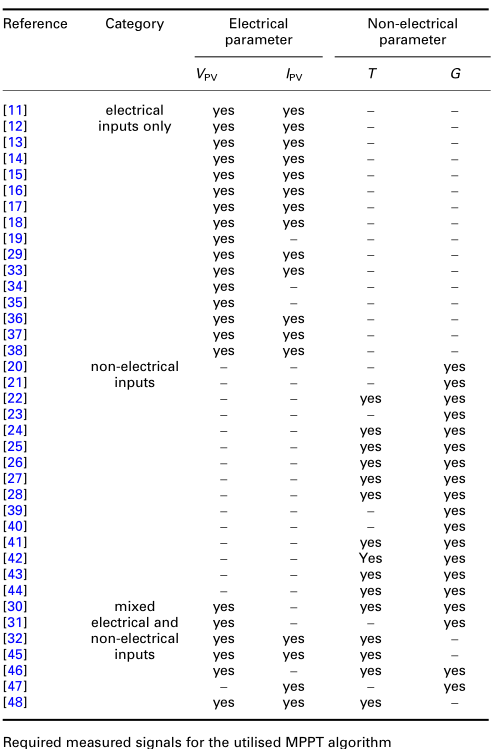
\includegraphics[width=.6\linewidth, height=6.5cm]{mppt.png}
        \caption{Required measured signals for the utilized MPPT algorithm.}
        \label{fig:mppt}
    \end{figure}
\end{frame}

\begin{frame}{Classification at a glance}
	\begin{figure}
    	\centering
        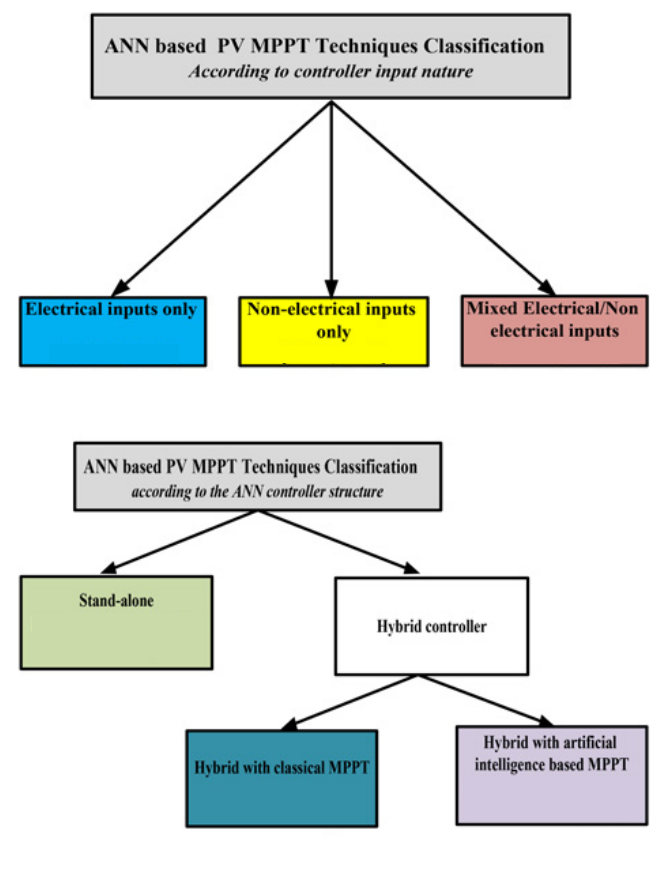
\includegraphics[width=.6\linewidth, height=6.5cm]{classification.png}
        \caption{Classification of MPPT Technique}
        \label{fig:classification}
    \end{figure}
\end{frame}

\begin{frame}[c, allowframebreaks]{According to Controller input nature}

ANN based PV MPPT Techniques can be classified into three categories based on controller input nature. 

\begin{enumerate}
	\item{Electrical inputs only (Figure \ref{fig:elecInput})}
    \item{Non-electrical inputs only (Figure \ref{fig:nonElecInput})}
    \item{Mixed Electrical/Non electrical inputs (Figure \ref{fig:mixedInput})}
\end{enumerate}

\framebreak 

\vspace{3.5cm}

\begin{figure}[b]
	\centering
	\centerline{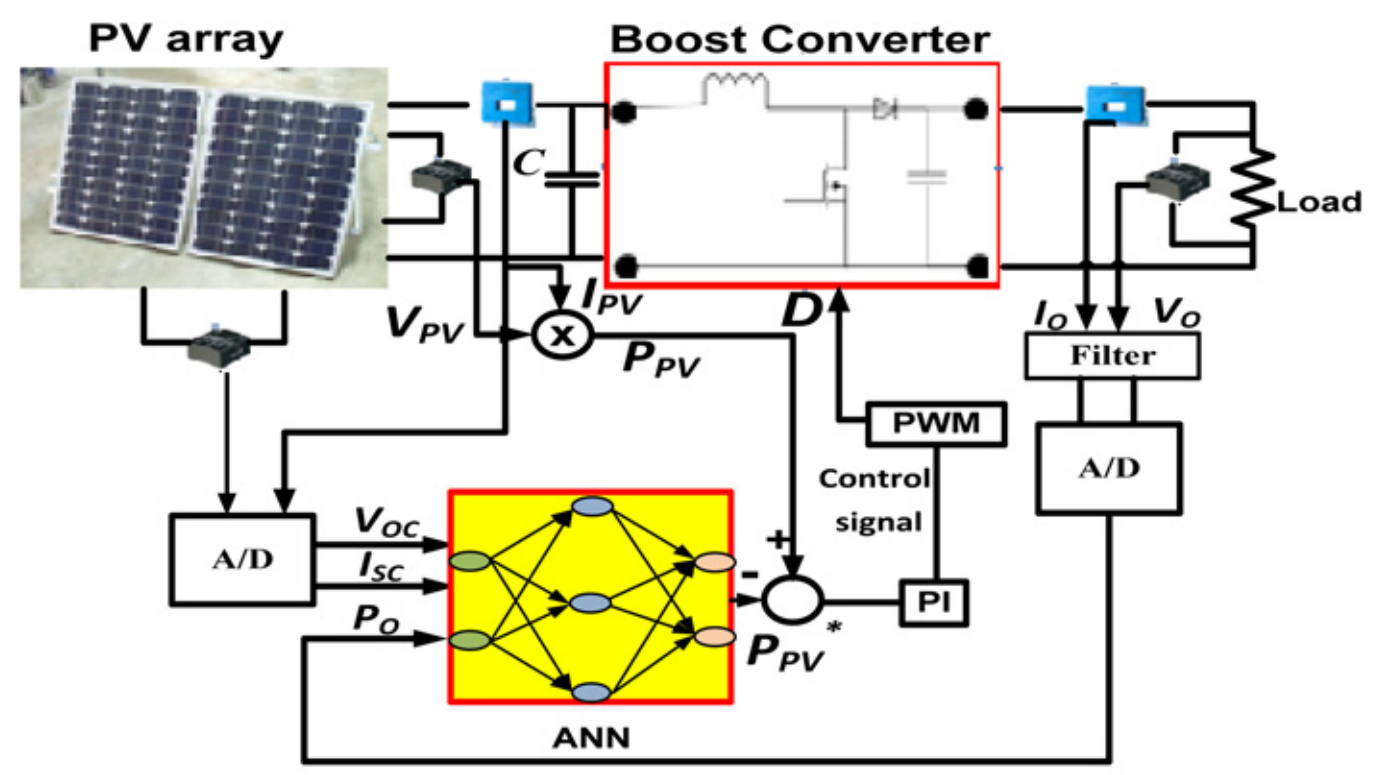
\includegraphics[scale=0.2]{elecinput.png}}
    \caption{MPPT technique with electrical inputs only.}
    \label{fig:elecInput}
\end{figure}

\framebreak 

\begin{figure}
	\centering
    \centerline{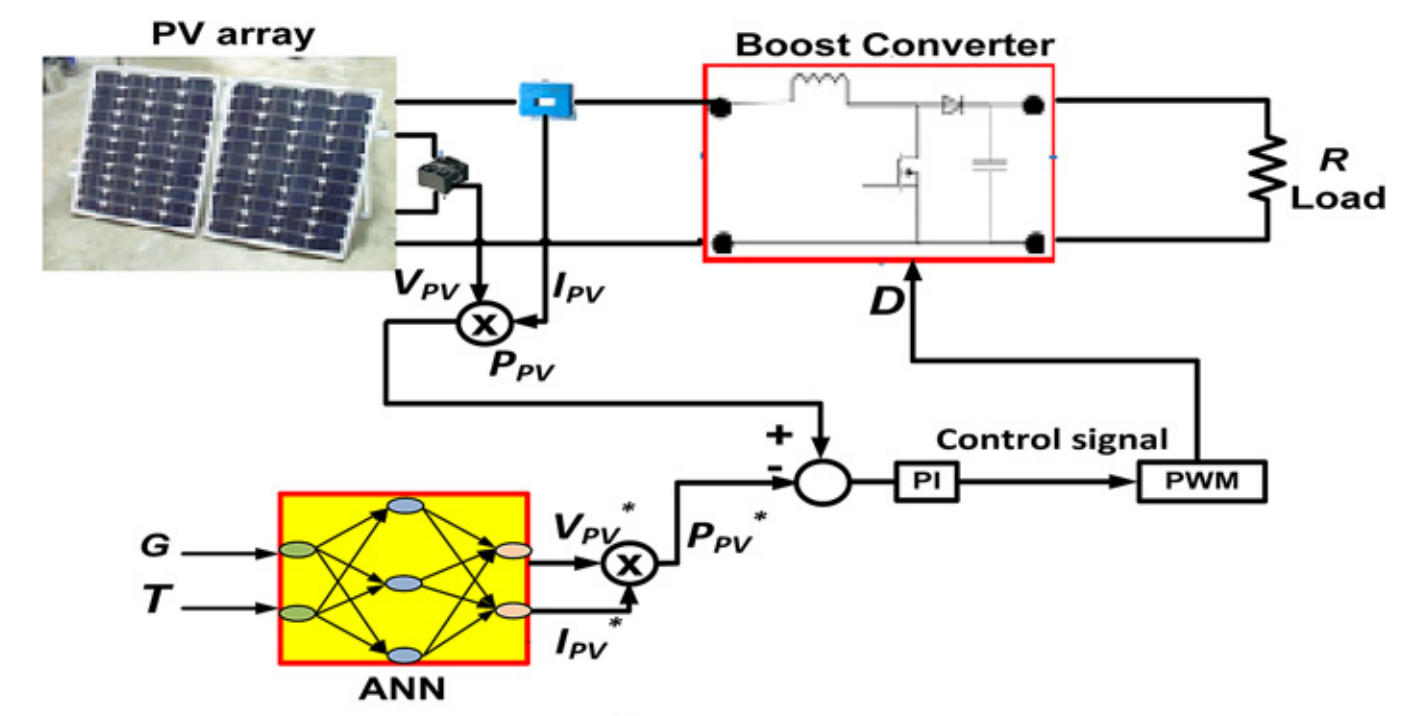
\includegraphics[scale=0.2]{nonelecinput.png}}
    \caption{MPPT technique with non electrical inputs only.}
    \label{fig:nonElecInput}
\end{figure}

\framebreak 

\begin{figure}
	\centerline{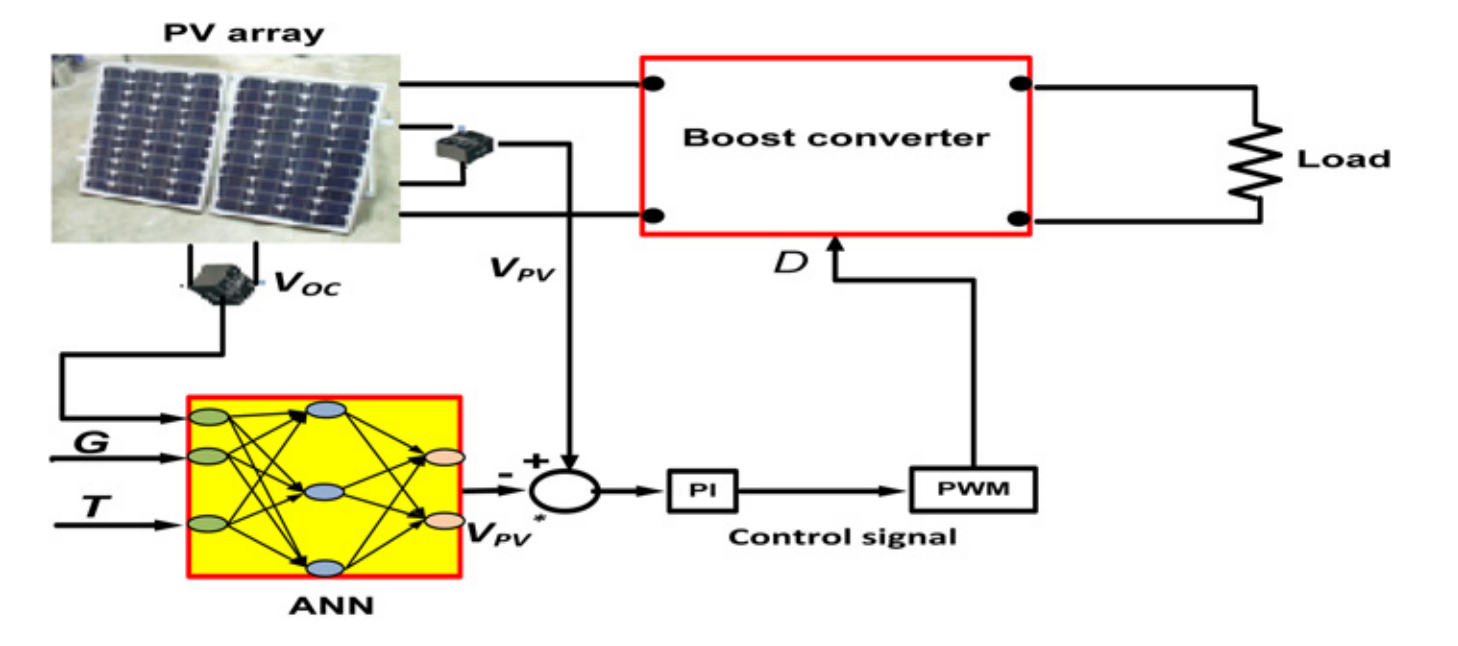
\includegraphics[scale=0.2]{mixedinput.png}}
    \caption{MPPT technique with mixed inputs only.}
    \label{fig:mixedInput}
\end{figure}
\end{frame}

% ANN Control structure based classification

\begin{frame}[c]{According to ANN Controller structure}

ANN based PV MPPT Techniques can be classified into two major categories based on \textit{ANN controller structure}. 

\textbf{Hybrid Controller} can be further classified into two categories.

\begin{enumerate}
	\item{Stand-alone (Figure \ref{fig:elecInput})}
    \item{Hybrid Controller
    	\begin{enumerate}
        	\item{Hybrid with Classical MPPT (Figure \ref{fig:hybridclassical})}
            \item{Hybrid with artificial intelligence based MPPT (Figure \ref{fig:hybridann})}
        \end{enumerate}
    }
\end{enumerate}

\end{frame}

\begin{frame}{MPPT with Classical technique}
\begin{figure}
	\centerline{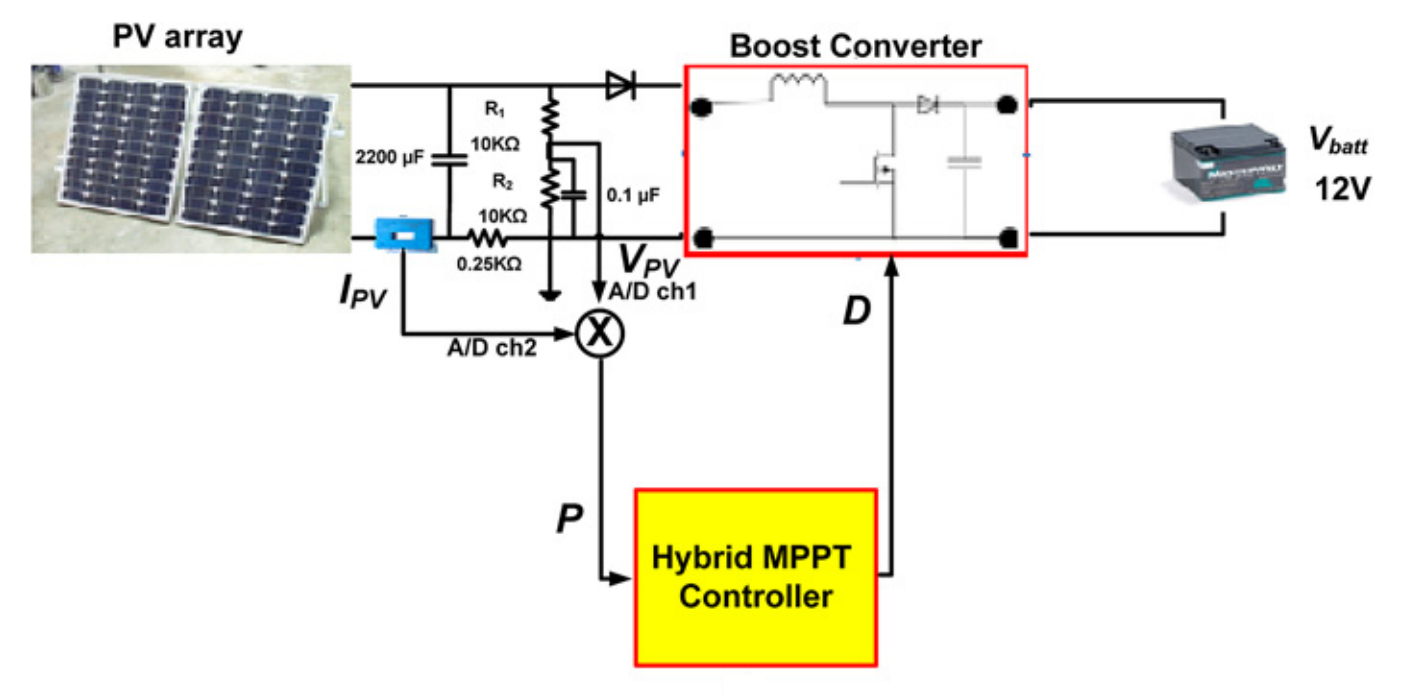
\includegraphics[scale=0.2]{hybridclassical.png}}
    \caption{ANN based PV MPPT Hybrid with classical MPPT technique.}
    \label{fig:hybridclassical}
\end{figure}
\end{frame}

\begin{frame}{MPPT with Artificial Intelligence technique}
\begin{figure}
	\centerline{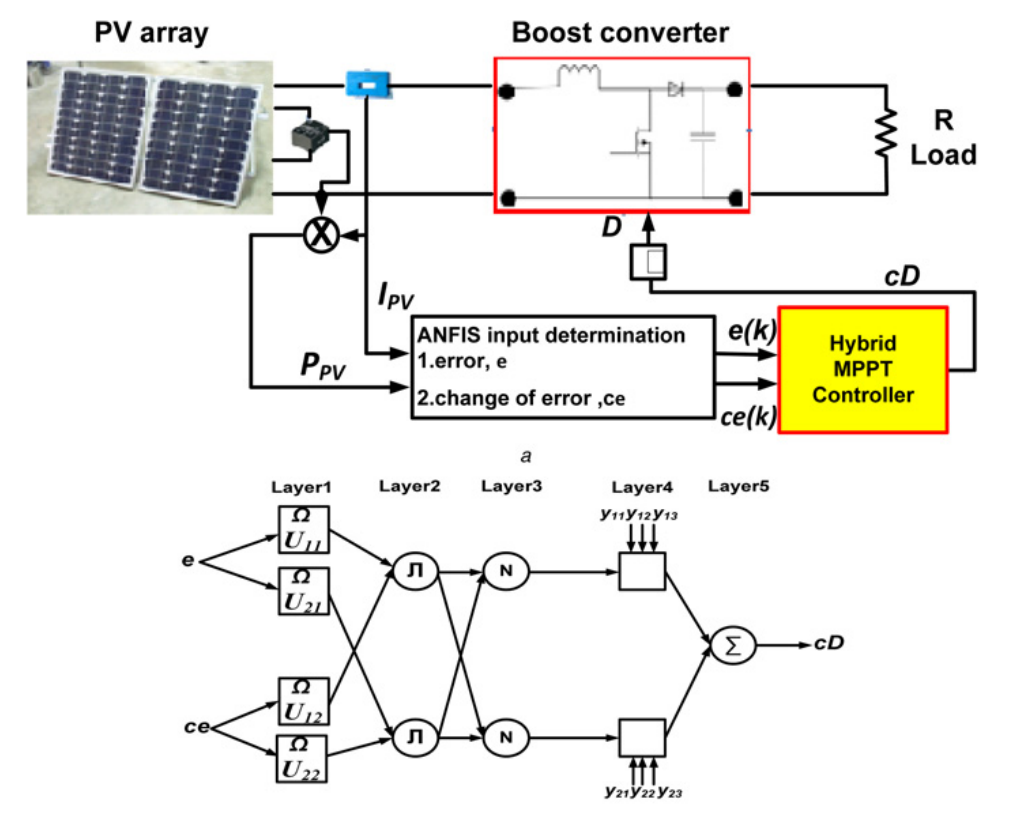
\includegraphics[scale=0.15]{hybridann.png}}
	\caption{ANN based PV MPPT Hybrid with artificial intelligence technique.}
    \label{fig:hybridann}
\end{figure}
\vspace{-1cm}
\begin{itemize}
	\item{High performance application}
    \item{Scarifying complexity}
\end{itemize}
We integrate the tracking operation with other artificial intelligence such as fuzzy logic, adaptive and genetic algorithms (GAs).
\end{frame}

\begin{frame}{Comparative Analysis}
	\begin{figure}
	\centerline{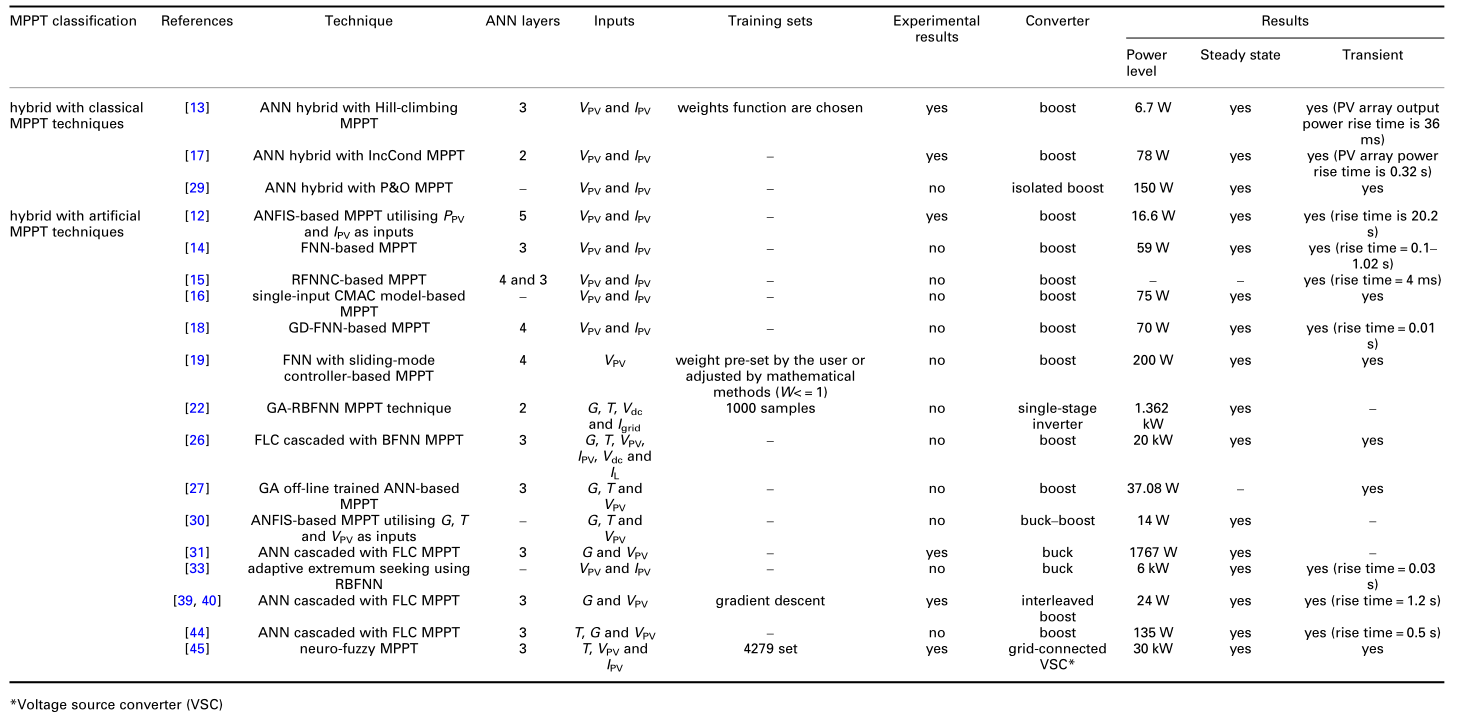
\includegraphics[scale=.23]{comparativeanalysis.png}}
	\caption{Comparison between MPPT classifications.}
    \label{fig:hybridann}
\end{figure}
\end{frame}

\begin{frame}{Conclusion}
\begin{alertblock}{All these techniques vary from different aspects,
such as:}
	\begin{itemize}
    	\item{Input signals}
        \item{Required measurements}
        \item{Complexity}
        \item{Computational burden}
        \item{Oscillation}
        \item{Transient}
        \item{Steady-state performance}
    \end{itemize}
\end{alertblock}
\end{frame}


\end{document}
